\subsection{Input Files}

At a minimum, one must specify 2 files for use in Puffin - a main input file, and a beam input file. The main file sets up the system scaling, the field mesh, the integration step sizes, and other simulation options. A simple, single undulator system can be setup here. It also specifies the names of the other input files, including the beam file.

The beam file specifies the electron beam parameters - there are 3 different types of beam input, detailed later in section \ref{beamfls}. Multiple beams can be specified, each with different characteristics, such as energies, lengths, charges, current profiles, etc.

Optionally, one may also supply a radiation seed file, to describe an injected radiation seed into the FEL with the electron beam. Similarly to the beam file, many radiation seeds can be specified here, at different frequencies, intensity profiles, \textit{etc}.

In addition, one may also supply a lattice file, which describes the layout of undulator modules, focusing quadrupoles, chicanes, drifts \textit{etc}. If this is not supplied, then a single undulator is set up as detailed in the main input file. If it is supplied, the wiggler in the main input file is ignored. Undulators can have independently variable polarizations, magnetic field strengths, etc. A description of available 3D undulator types is available in section \ref{und-fields}.

The main input file sets the frequency of data dumps from Puffin. Additionally, a `write file' can be supplied to give more flexibility and specify exactly when the data is written.

Puffin can be resumed from a previous run - if your cluster crashes, for instance. You could even resume from a previous run to extend or change undulator parameters, for instance.

Figure \ref{inputs1} shows a schematic of the Puffin input decks. Puffin comes with a few example input decks for reference.

\begin{figure*}
\centering
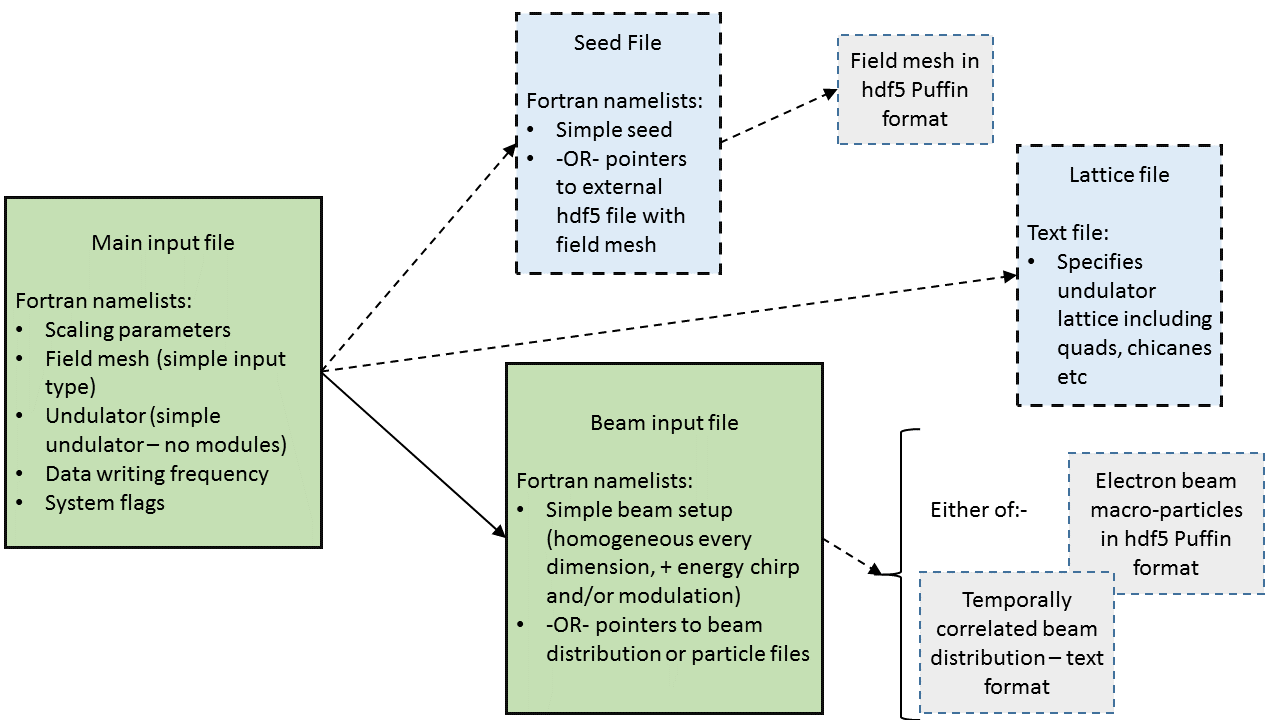
\includegraphics[width=120mm]{InputFiles.png}
\caption{Schematic of input files - dashed lines indicate optional files.}
\label{inputs1}
\end{figure*}